\scanpage{29}
% archive foliation: 28
\uline{Définition} 1. Soient $X$ un préschéma \deleted{\unsure{de}} sur un corps $k$, $F_i$ \deleted{et $G$} $(i=1,2)$ un faisceau algébrique sur $X_i=X\otimes_kK_i$, où $K_i$ est une extension de $k$. On dit que $F_1$ et $F_2$ sont \uline{$\unsure{K|k}$-équivalents} s'il existe une extension $K'$ de $k$, des $k$-hom $u_i:K_i\longrightarrow K'$, tels que \deleted{un isomorphisme} les faisceaux algébriques \inserted{$F_i\otimes_{K_i}K'$} sur $X\otimes_kK'\simeq X_i\otimes_{K_i}K'$ soient isomorphes. \deleted{Les classes d'équivalence} Classes géométriques de faisceaux.
\figure{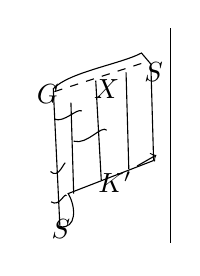
\begin{tikzpicture}[scale=.7]
\draw (0,0)..controls (.3,-.05) and (.3,.35)..(.15,.6)--(1.7,1.2);
\draw (0,0)--(-.12,2.5)..controls (.15,2.8) and (1.1,2.95)..(1.48,3.15)--(1.65,2.95)--(1.7,1.2);
\draw[dashed] (-.1,2.45)--(1.6,3);
\draw (.25,.6)--(.2,2.25);\draw (.75,.85)--(.65,2.65);\draw (1.25,1.05)--(1.2,2.8);
\draw (-.1,1.95)..controls (.08,1.88) and (.3,2.15)..(.4,2.1);
\draw (.25,1.55)..controls (.5,1.48) and (.75,1.85)..(.85,1.75);
\draw (-.17,1)..controls (-.02,.85) and (.08,1.2)..(.1,1.15);
\draw (-.16,.45)..controls (0,.35) and (.08,.63)..(.12,.56);
\draw[->] (1.4,1.1)--(1.75,1.3);
\node at (.85,2.5) {$X$};\node at (1,.8) {$K'$};
\node at (-.22,2.4) {$\unsure{G}$};\node at (1.7,2.8) {$\unsure{S}$};\node at (.02,-.05) {$\unsure{S}$};
\draw (2,3.6)--(2,-.3);
\end{tikzpicture}}

On vérifie facilement que c'est là une \uline{relation d'équivalence} entre \deleted{faisceaux}\inserted{couples $(K,F)$} d'une ext. $K$ de $k$ et d'un faisceau algébrique $F$ sur $X\otimes_kK$, en vertu du fait de transitivité de l'extension des scalaires et du fait que deux extensions de $k$ peuvent toujours être ``dominées'' par une troisième.

\uline{Proposition 2} \inserted{Si $X$ est de type fini sur $k$,} Tout faisceau cohérent sur un $X\otimes_kK$ est équivalent à un faisceau algébrique sur un $X\otimes_kK'$, où $K'$ est une ss-extension de $K$ de type fini sur $k$.

Si $F_1$ sur $X\otimes_kK_1$ et $F_2$ sur $X\otimes_kK_2$ sont des faisceaux cohérents \uline{équivalents}, \deleted{\unsure{alors}}\inserted{les $K_i$ de type fini sur $k$,} \deleted{\unsure{deux de type fini}} alors dans
